% Options for packages loaded elsewhere
\PassOptionsToPackage{unicode}{hyperref}
\PassOptionsToPackage{hyphens}{url}
%
\documentclass[
]{book}
\usepackage{lmodern}
\usepackage{amssymb,amsmath}
\usepackage{ifxetex,ifluatex}
\ifnum 0\ifxetex 1\fi\ifluatex 1\fi=0 % if pdftex
  \usepackage[T1]{fontenc}
  \usepackage[utf8]{inputenc}
  \usepackage{textcomp} % provide euro and other symbols
\else % if luatex or xetex
  \usepackage{unicode-math}
  \defaultfontfeatures{Scale=MatchLowercase}
  \defaultfontfeatures[\rmfamily]{Ligatures=TeX,Scale=1}
\fi
% Use upquote if available, for straight quotes in verbatim environments
\IfFileExists{upquote.sty}{\usepackage{upquote}}{}
\IfFileExists{microtype.sty}{% use microtype if available
  \usepackage[]{microtype}
  \UseMicrotypeSet[protrusion]{basicmath} % disable protrusion for tt fonts
}{}
\makeatletter
\@ifundefined{KOMAClassName}{% if non-KOMA class
  \IfFileExists{parskip.sty}{%
    \usepackage{parskip}
  }{% else
    \setlength{\parindent}{0pt}
    \setlength{\parskip}{6pt plus 2pt minus 1pt}}
}{% if KOMA class
  \KOMAoptions{parskip=half}}
\makeatother
\usepackage{xcolor}
\IfFileExists{xurl.sty}{\usepackage{xurl}}{} % add URL line breaks if available
\IfFileExists{bookmark.sty}{\usepackage{bookmark}}{\usepackage{hyperref}}
\hypersetup{
  pdftitle={AQP Examples},
  pdfauthor={Hava Blair},
  hidelinks,
  pdfcreator={LaTeX via pandoc}}
\urlstyle{same} % disable monospaced font for URLs
\usepackage{color}
\usepackage{fancyvrb}
\newcommand{\VerbBar}{|}
\newcommand{\VERB}{\Verb[commandchars=\\\{\}]}
\DefineVerbatimEnvironment{Highlighting}{Verbatim}{commandchars=\\\{\}}
% Add ',fontsize=\small' for more characters per line
\usepackage{framed}
\definecolor{shadecolor}{RGB}{248,248,248}
\newenvironment{Shaded}{\begin{snugshade}}{\end{snugshade}}
\newcommand{\AlertTok}[1]{\textcolor[rgb]{0.94,0.16,0.16}{#1}}
\newcommand{\AnnotationTok}[1]{\textcolor[rgb]{0.56,0.35,0.01}{\textbf{\textit{#1}}}}
\newcommand{\AttributeTok}[1]{\textcolor[rgb]{0.77,0.63,0.00}{#1}}
\newcommand{\BaseNTok}[1]{\textcolor[rgb]{0.00,0.00,0.81}{#1}}
\newcommand{\BuiltInTok}[1]{#1}
\newcommand{\CharTok}[1]{\textcolor[rgb]{0.31,0.60,0.02}{#1}}
\newcommand{\CommentTok}[1]{\textcolor[rgb]{0.56,0.35,0.01}{\textit{#1}}}
\newcommand{\CommentVarTok}[1]{\textcolor[rgb]{0.56,0.35,0.01}{\textbf{\textit{#1}}}}
\newcommand{\ConstantTok}[1]{\textcolor[rgb]{0.00,0.00,0.00}{#1}}
\newcommand{\ControlFlowTok}[1]{\textcolor[rgb]{0.13,0.29,0.53}{\textbf{#1}}}
\newcommand{\DataTypeTok}[1]{\textcolor[rgb]{0.13,0.29,0.53}{#1}}
\newcommand{\DecValTok}[1]{\textcolor[rgb]{0.00,0.00,0.81}{#1}}
\newcommand{\DocumentationTok}[1]{\textcolor[rgb]{0.56,0.35,0.01}{\textbf{\textit{#1}}}}
\newcommand{\ErrorTok}[1]{\textcolor[rgb]{0.64,0.00,0.00}{\textbf{#1}}}
\newcommand{\ExtensionTok}[1]{#1}
\newcommand{\FloatTok}[1]{\textcolor[rgb]{0.00,0.00,0.81}{#1}}
\newcommand{\FunctionTok}[1]{\textcolor[rgb]{0.00,0.00,0.00}{#1}}
\newcommand{\ImportTok}[1]{#1}
\newcommand{\InformationTok}[1]{\textcolor[rgb]{0.56,0.35,0.01}{\textbf{\textit{#1}}}}
\newcommand{\KeywordTok}[1]{\textcolor[rgb]{0.13,0.29,0.53}{\textbf{#1}}}
\newcommand{\NormalTok}[1]{#1}
\newcommand{\OperatorTok}[1]{\textcolor[rgb]{0.81,0.36,0.00}{\textbf{#1}}}
\newcommand{\OtherTok}[1]{\textcolor[rgb]{0.56,0.35,0.01}{#1}}
\newcommand{\PreprocessorTok}[1]{\textcolor[rgb]{0.56,0.35,0.01}{\textit{#1}}}
\newcommand{\RegionMarkerTok}[1]{#1}
\newcommand{\SpecialCharTok}[1]{\textcolor[rgb]{0.00,0.00,0.00}{#1}}
\newcommand{\SpecialStringTok}[1]{\textcolor[rgb]{0.31,0.60,0.02}{#1}}
\newcommand{\StringTok}[1]{\textcolor[rgb]{0.31,0.60,0.02}{#1}}
\newcommand{\VariableTok}[1]{\textcolor[rgb]{0.00,0.00,0.00}{#1}}
\newcommand{\VerbatimStringTok}[1]{\textcolor[rgb]{0.31,0.60,0.02}{#1}}
\newcommand{\WarningTok}[1]{\textcolor[rgb]{0.56,0.35,0.01}{\textbf{\textit{#1}}}}
\usepackage{longtable,booktabs}
% Correct order of tables after \paragraph or \subparagraph
\usepackage{etoolbox}
\makeatletter
\patchcmd\longtable{\par}{\if@noskipsec\mbox{}\fi\par}{}{}
\makeatother
% Allow footnotes in longtable head/foot
\IfFileExists{footnotehyper.sty}{\usepackage{footnotehyper}}{\usepackage{footnote}}
\makesavenoteenv{longtable}
\usepackage{graphicx}
\makeatletter
\def\maxwidth{\ifdim\Gin@nat@width>\linewidth\linewidth\else\Gin@nat@width\fi}
\def\maxheight{\ifdim\Gin@nat@height>\textheight\textheight\else\Gin@nat@height\fi}
\makeatother
% Scale images if necessary, so that they will not overflow the page
% margins by default, and it is still possible to overwrite the defaults
% using explicit options in \includegraphics[width, height, ...]{}
\setkeys{Gin}{width=\maxwidth,height=\maxheight,keepaspectratio}
% Set default figure placement to htbp
\makeatletter
\def\fps@figure{htbp}
\makeatother
\setlength{\emergencystretch}{3em} % prevent overfull lines
\providecommand{\tightlist}{%
  \setlength{\itemsep}{0pt}\setlength{\parskip}{0pt}}
\setcounter{secnumdepth}{5}
\usepackage{booktabs}
\usepackage{amsthm}
\makeatletter
\def\thm@space@setup{%
  \thm@preskip=8pt plus 2pt minus 4pt
  \thm@postskip=\thm@preskip
}
\makeatother
\usepackage[]{natbib}
\bibliographystyle{apalike}

\title{AQP Examples}
\author{Hava Blair}
\date{2020-09-06}

\begin{document}
\maketitle

{
\setcounter{tocdepth}{1}
\tableofcontents
}
\hypertarget{prerequisites}{%
\chapter{Prerequisites}\label{prerequisites}}

This is a \emph{sample} book written in \textbf{Markdown}. You can use anything that Pandoc's Markdown supports, e.g., a math equation \(a^2 + b^2 = c^2\).

The \textbf{aqp} package can be installed from CRAN:

\begin{Shaded}
\begin{Highlighting}[]
\CommentTok{\#install.packages("aqp")}
\CommentTok{\# or the development version}
\CommentTok{\# devtools::install\_github("ncss{-}tech/aqp")}
\end{Highlighting}
\end{Shaded}

Remember each Rmd file contains one and only one chapter, and a chapter is defined by the first-level heading \texttt{\#}.

To compile this example to PDF, you need XeLaTeX. You are recommended to install TinyTeX (which includes XeLaTeX): \url{https://yihui.name/tinytex/}.

\hypertarget{waseca-soil-pits}{%
\chapter{Waseca Soil Pits}\label{waseca-soil-pits}}

date: 2020-07-11

\begin{Shaded}
\begin{Highlighting}[]
\NormalTok{knitr}\OperatorTok{::}\NormalTok{opts\_chunk}\OperatorTok{$}\KeywordTok{set}\NormalTok{(}\DataTypeTok{echo =} \OtherTok{TRUE}\NormalTok{)}
\KeywordTok{library}\NormalTok{(dplyr)}
\KeywordTok{library}\NormalTok{(readxl)}
\KeywordTok{library}\NormalTok{(aqp)}
\KeywordTok{library}\NormalTok{(munsell)}
\KeywordTok{library}\NormalTok{(soilDB)}
\end{Highlighting}
\end{Shaded}

\hypertarget{about}{%
\section{About}\label{about}}

Soil pits in Vivian Township, Waseca County, MN. Just north of Faribault county line. Visited July 8, 2020 for filming of UMN Extension educational video on soil structure.

Pea field with 2 pits dug by cooperator. First pit in the headlands where pea health was very poor. Second pit directly north \textasciitilde30m from headland pit.

Field pit slightly upland from headland pit. Cattails visible in field corner not far from headlands pit - clearly a wet area. Field tiled for drainage, tile \textasciitilde3 feet deep in this area.

\hypertarget{headlands-pit}{%
\subsection{Headlands Pit}\label{headlands-pit}}

Canisteo? Official Series Description \href{https://soilseries.sc.egov.usda.gov/OSD_Docs/C/CANISTEO.html}{here}

Located at 43.8483, -93.6614

\hypertarget{field-pit}{%
\subsection{Field Pit}\label{field-pit}}

Nicollet? Official Series Description \href{https://soilseries.sc.egov.usda.gov/OSD_Docs/N/NICOLLET.html}{here}

Located at 43.8487, -93.6614

\hypertarget{description-data-collected}{%
\section{Description data collected}\label{description-data-collected}}

\begin{verbatim}
##     PedonID           id hzname top bottom  hue value chroma Texture HzID    Effervescence
## 1  Headland Pit-Canisteo     Ap   0     20    N   2.0      0     SiC    1               NA
## 2  Headland Pit-Canisteo      A  20     30    N   2.0      0     SiC    2               SL
## 3  Headland Pit-Canisteo     BA  30     40 2.5Y   3.0      1      CL    3               ST
## 4  Headland Pit-Canisteo    Bkg  40     70 2.5Y   6.0      2      CL    4               ST
## 5  Headland Pit-Canisteo      C  70    100 2.5Y   6.0      2      CL    5               ST
## 6     Field Pit-Nicollet     Ap   0     30 10YR   2.0      1      CL    6               NA
## 7     Field Pit-Nicollet      A  30     50 2.5Y   2.5      1      CL    7               NA
## 8     Field Pit-Nicollet     Bw  50     70 2.5Y   3.0      2      CL    8               NA
## 9     Field Pit-Nicollet    Bg?  70     90 2.5Y   4.0      2      CL    9               NA
## 10    Field Pit-Nicollet      C  90    110 2.5Y   4.0      3       L   10 ST - masses only
\end{verbatim}

\begin{verbatim}
##     PedonID           id hzname
## 1  Headland Pit-Canisteo     Ap
## 2  Headland Pit-Canisteo      A
## 3  Headland Pit-Canisteo     BA
## 4  Headland Pit-Canisteo    Bkg
## 5  Headland Pit-Canisteo      C
## 6     Field Pit-Nicollet     Ap
## 7     Field Pit-Nicollet      A
## 8     Field Pit-Nicollet     Bw
## 9     Field Pit-Nicollet    Bg?
## 10    Field Pit-Nicollet      C
##                                                                             Redox
## 1                                                                            <NA>
## 2                                                                            <NA>
## 3                                                                            <NA>
## 4                                                                            <NA>
## 5                                         Common, fine & medium Fe conc 7.5YR 5/8
## 6                                                                            <NA>
## 7                                                                            <NA>
## 8                                                                            <NA>
## 9                                                      Few fine Fe conc 7.5YR 5/8
## 10 Common fine Fe conc 7.5YR 5/8; some pockets of Fe-stained coarse sand & gravel
\end{verbatim}

\begin{verbatim}
##     PedonID           id hzname
## 1  Headland Pit-Canisteo     Ap
## 2  Headland Pit-Canisteo      A
## 3  Headland Pit-Canisteo     BA
## 4  Headland Pit-Canisteo    Bkg
## 5  Headland Pit-Canisteo      C
## 6     Field Pit-Nicollet     Ap
## 7     Field Pit-Nicollet      A
## 8     Field Pit-Nicollet     Bw
## 9     Field Pit-Nicollet    Bg?
## 10    Field Pit-Nicollet      C
##                                                                                                                              Notes
## 1                                                                                                                             <NA>
## 2                                                                                                                             <NA>
## 3                                                                                                                             <NA>
## 4                                                                                                                             <NA>
## 5                                                                                                                             <NA>
## 6                                                                                                                             <NA>
## 7                                                                                                                             <NA>
## 8                                                                                                                             <NA>
## 9                                                                                                                             <NA>
## 10 A few limestone coarse fragments 4-6cm in diameter; some carbonate masses that effervesce strongly, but overall matrix does not
\end{verbatim}

\hypertarget{create-soilprofilecollection-spc-objects}{%
\section{Create SoilProfileCollection (SPC) objects}\label{create-soilprofilecollection-spc-objects}}

\begin{Shaded}
\begin{Highlighting}[]
\CommentTok{\# promote data\_min\_st dataframe to SoilProfileCollection }
\KeywordTok{depths}\NormalTok{(data\_pits) \textless{}{-}}\StringTok{ }\NormalTok{id }\OperatorTok{\textasciitilde{}}\StringTok{ }\NormalTok{top }\OperatorTok{+}\StringTok{ }\NormalTok{bottom}

\CommentTok{\#check that we have successfully converted class to SPC}
\KeywordTok{class}\NormalTok{(data\_pits)}
\end{Highlighting}
\end{Shaded}

\begin{verbatim}
## [1] "SoilProfileCollection"
## attr(,"package")
## [1] "aqp"
\end{verbatim}

\begin{Shaded}
\begin{Highlighting}[]
\CommentTok{\# OSD data for the two series I think we have at the Waseca pits}
\NormalTok{osd\_pedons \textless{}{-}}\StringTok{ }\KeywordTok{fetchOSD}\NormalTok{(}\KeywordTok{c}\NormalTok{(}\StringTok{\textquotesingle{}canisteo\textquotesingle{}}\NormalTok{, }\StringTok{\textquotesingle{}nicollet\textquotesingle{}}\NormalTok{))}
\end{Highlighting}
\end{Shaded}

\hypertarget{visually-compare-field-descriptions-with-osds}{%
\section{Visually compare field descriptions with OSDs}\label{visually-compare-field-descriptions-with-osds}}

\begin{Shaded}
\begin{Highlighting}[]
\CommentTok{\# join the OSD pedons with the pit pedons}
\NormalTok{both \textless{}{-}}\StringTok{ }\NormalTok{aqp}\OperatorTok{::}\KeywordTok{union}\NormalTok{(}\KeywordTok{list}\NormalTok{(osd\_pedons, data\_pits))}

\CommentTok{\# set margins}
\KeywordTok{par}\NormalTok{(}\DataTypeTok{mar =} \KeywordTok{c}\NormalTok{(}\DecValTok{5}\NormalTok{,}\DecValTok{3}\NormalTok{,}\DecValTok{2}\NormalTok{,}\DecValTok{2}\NormalTok{), }\DataTypeTok{xpd=}\OtherTok{NA}\NormalTok{)}

\CommentTok{\# plot soil profile collection}
\KeywordTok{plotSPC}\NormalTok{(both, }\DataTypeTok{width =} \FloatTok{0.25}\NormalTok{, }\DataTypeTok{name =} \StringTok{\textquotesingle{}hzname\textquotesingle{}}\NormalTok{, }\DataTypeTok{plot.order=} \KeywordTok{c}\NormalTok{(}\DecValTok{1}\NormalTok{,}\DecValTok{3}\NormalTok{,}\DecValTok{2}\NormalTok{,}\DecValTok{4}\NormalTok{), }\DataTypeTok{cex.names =} \FloatTok{0.7}\NormalTok{)}
\end{Highlighting}
\end{Shaded}

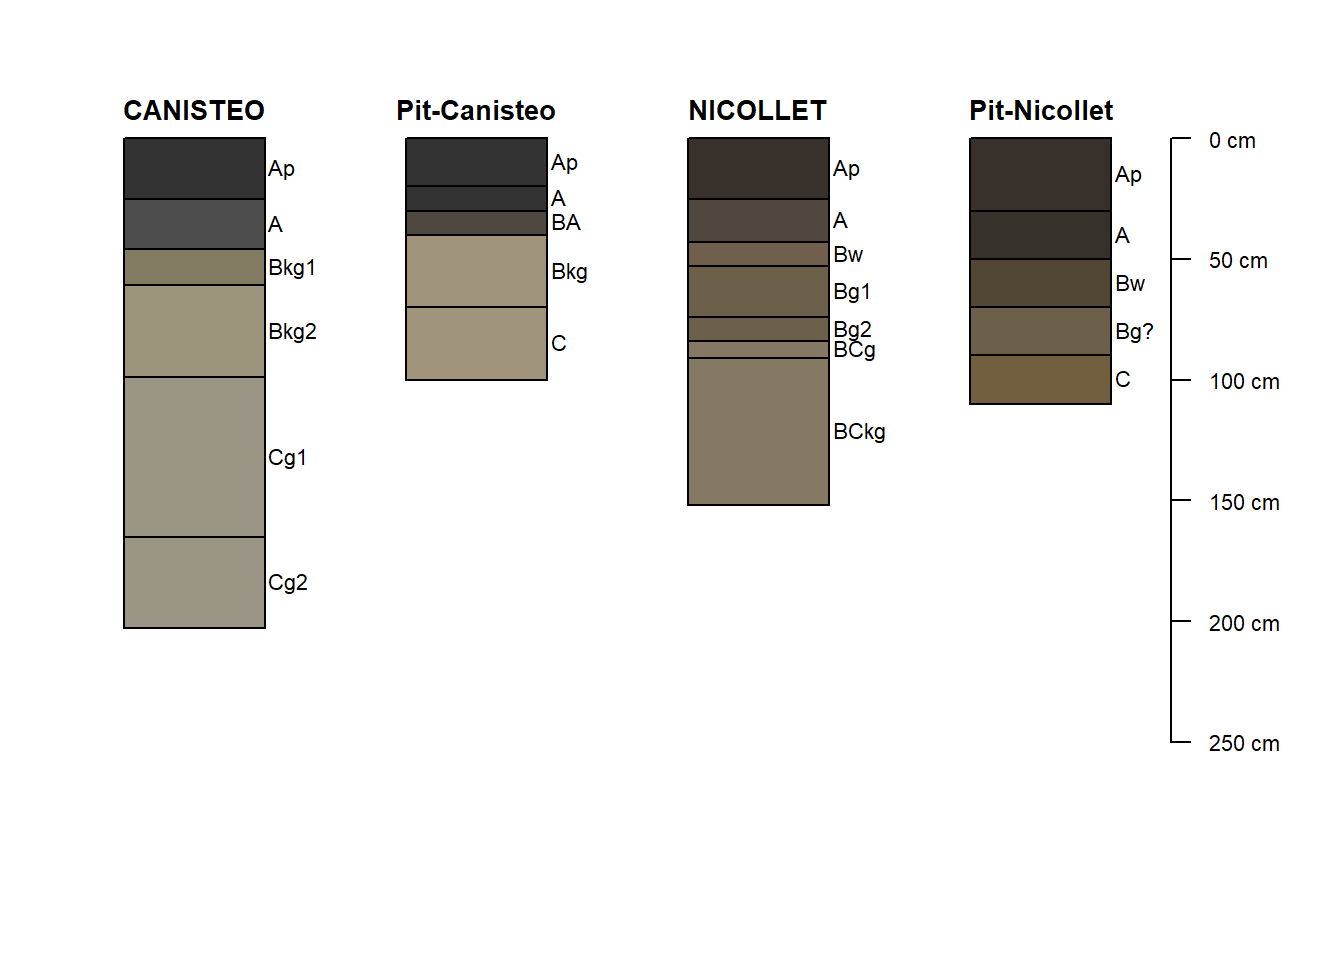
\includegraphics{bookdown-demo_files/figure-latex/pedon-plot-1.pdf}

\hypertarget{mower-county-pedons}{%
\chapter{Mower County Pedons}\label{mower-county-pedons}}

date: 2020-09-06

\hypertarget{overview}{%
\section{Overview}\label{overview}}

Visualizing some soil profile descriptions from SL in Mower County.

This SPC plotting ideas post was helpful but I had to dig in the documentation to find it - not linked on the main aqp webpage?
\url{http://ncss-tech.github.io/AQP/aqp/SPC-plotting-ideas.html}

\begin{Shaded}
\begin{Highlighting}[]
\NormalTok{knitr}\OperatorTok{::}\NormalTok{opts\_chunk}\OperatorTok{$}\KeywordTok{set}\NormalTok{(}\DataTypeTok{echo =} \OtherTok{TRUE}\NormalTok{)}
\NormalTok{knitr}\OperatorTok{::}\NormalTok{opts\_chunk}\OperatorTok{$}\KeywordTok{set}\NormalTok{(}\DataTypeTok{tidy =} \OtherTok{TRUE}\NormalTok{)}
\NormalTok{knitr}\OperatorTok{::}\NormalTok{opts\_chunk}\OperatorTok{$}\KeywordTok{set}\NormalTok{(}\DataTypeTok{tidy.opts =} \KeywordTok{list}\NormalTok{(}\DataTypeTok{width.cutoff=}\DecValTok{60}\NormalTok{))}

\KeywordTok{library}\NormalTok{(tidyverse)}
\KeywordTok{library}\NormalTok{(aqp)}
\KeywordTok{library}\NormalTok{(readxl)}
\KeywordTok{library}\NormalTok{(munsell)}
\end{Highlighting}
\end{Shaded}

\hypertarget{load-data}{%
\section{Load data}\label{load-data}}

\begin{Shaded}
\begin{Highlighting}[]
\NormalTok{pedons \textless{}{-}}\StringTok{ }\KeywordTok{read\_excel}\NormalTok{(}\StringTok{"./data/mower\_pedons.xlsx"}\NormalTok{) }\OperatorTok{\%\textgreater{}\%}\StringTok{ }\KeywordTok{as.data.frame}\NormalTok{()}

\NormalTok{sites \textless{}{-}}\StringTok{ }\KeywordTok{read\_excel}\NormalTok{(}\StringTok{"./data/mower\_site.xlsx"}\NormalTok{)}
\end{Highlighting}
\end{Shaded}

\hypertarget{munsell-colors-conversion}{%
\section{Munsell colors conversion}\label{munsell-colors-conversion}}

\begin{Shaded}
\begin{Highlighting}[]
\CommentTok{\# convert munsell colors to R compatible colors and add}
\CommentTok{\# horizon ID}
\NormalTok{with\_colors \textless{}{-}}\StringTok{ }\NormalTok{pedons }\OperatorTok{\%\textgreater{}\%}\StringTok{ }\KeywordTok{mutate}\NormalTok{(}\DataTypeTok{soil\_color =} \KeywordTok{munsell2rgb}\NormalTok{(hue, }
\NormalTok{    value, chroma), }\DataTypeTok{hzID =} \KeywordTok{c}\NormalTok{(}\DecValTok{1}\OperatorTok{:}\KeywordTok{nrow}\NormalTok{(pedons)))}

\NormalTok{with\_colors}
\end{Highlighting}
\end{Shaded}

\begin{verbatim}
##        id top bottom name  hue value chroma soil_color hzID
## 1  1CVA-8   0      2   A1 2.5Y   2.5      1  #36312BFF    1
## 2  1CVA-8   2      3   A2 2.5Y   2.5      1  #36312BFF    2
## 3  1CVA-8   3      7   A3 2.5Y   2.5      1  #36312BFF    3
## 4  1CVA-8   7      8   A4 2.5Y   3.0      2  #524735FF    4
## 5  1CVA-8   8     12   B1 2.5Y   4.0      2  #6C604AFF    5
## 6  1CVA-8  12     13  2B2 2.5Y   4.0      2  #6C604AFF    6
## 7  1CVA-8  13     20  2B3 2.5Y   4.0      2  #6C604AFF    7
## 8  1CVA-8  20     37  2B4 10YR   5.0      2  #897866FF    8
## 9  1CVA-8  37     45  2BC 10YR   5.0      1  #83796FFF    9
## 10 1BMA-4   0      6   A1 10YR   2.0      1  #38302AFF   10
## 11 1BMA-4   6     11   A2 10YR   2.0      1  #38302AFF   11
## 12 1BMA-4  11     18   A3 10YR   2.0      2  #3D2F21FF   12
## 13 1BMA-4  18     21   A4 10YR   3.0      2  #554636FF   13
## 14 1BMA-4  21     25   B1 10YR   4.0      3  #755D41FF   14
## 15 1BMA-4  25     32  2B2 10YR   5.0      2  #897866FF   15
## 16 1BMA-4  32     51  2B3 10YR   5.0      2  #897866FF   16
## 17 1BMA-4  51     60  2BC 10YR   5.0      2  #897866FF   17
## 18 1SHA-1   0      1   A1 10YR   2.0      2  #3D2F21FF   18
## 19 1SHA-1   1      4   A2 10YR   2.0      2  #3D2F21FF   19
## 20 1SHA-1   4      8   A3 10YR   2.0      2  #3D2F21FF   20
## 21 1SHA-1   8     10   B1 10YR   4.0      3  #755D41FF   21
## 22 1SHA-1  10     15  2B2 10YR   4.0      3  #755D41FF   22
## 23 1SHA-1  15     24  2B3 10YR   4.0      2  #6F5F4CFF   23
## 24 1SHA-1  24     40  2B4 10YR   5.0      2  #897866FF   24
## 25 1SHA-1  40     45  2BC 10YR   5.0      2  #897866FF   25
\end{verbatim}

\hypertarget{promote-dataframe-to-spc-object}{%
\section{Promote dataframe to SPC object}\label{promote-dataframe-to-spc-object}}

SPC = soil profile collection (S4 object)

\begin{Shaded}
\begin{Highlighting}[]
\CommentTok{\# promote dataframe to SPC object}
\KeywordTok{depths}\NormalTok{(with\_colors) \textless{}{-}}\StringTok{ }\NormalTok{id }\OperatorTok{\textasciitilde{}}\StringTok{ }\NormalTok{top }\OperatorTok{+}\StringTok{ }\NormalTok{bottom}
\end{Highlighting}
\end{Shaded}

\begin{verbatim}
## using `hzID` as a unique horizon ID
\end{verbatim}

\begin{Shaded}
\begin{Highlighting}[]
\CommentTok{\# should be \textquotesingle{}SoilProfileCollection\textquotesingle{}}
\KeywordTok{class}\NormalTok{(with\_colors)}
\end{Highlighting}
\end{Shaded}

\begin{verbatim}
## [1] "SoilProfileCollection"
## attr(,"package")
## [1] "aqp"
\end{verbatim}

\begin{Shaded}
\begin{Highlighting}[]
\CommentTok{\# inspect output}
\KeywordTok{str}\NormalTok{(with\_colors)}
\end{Highlighting}
\end{Shaded}

\begin{verbatim}
## Formal class 'SoilProfileCollection' [package "aqp"] with 11 slots
##   ..@ idcol       : chr "id"
##   ..@ hzidcol     : chr "hzID"
##   ..@ hzdesgncol  : chr(0) 
##   ..@ hztexclcol  : chr(0) 
##   ..@ depthcols   : chr [1:2] "top" "bottom"
##   ..@ metadata    :'data.frame':	1 obs. of  1 variable:
##   .. ..$ depth_units: chr "cm"
##   ..@ horizons    :'data.frame':	25 obs. of  9 variables:
##   .. ..$ id        : chr [1:25] "1BMA-4" "1BMA-4" "1BMA-4" "1BMA-4" ...
##   .. ..$ top       : num [1:25] 0 6 11 18 21 25 32 51 0 2 ...
##   .. ..$ bottom    : num [1:25] 6 11 18 21 25 32 51 60 2 3 ...
##   .. ..$ name      : chr [1:25] "A1" "A2" "A3" "A4" ...
##   .. ..$ hue       : chr [1:25] "10YR" "10YR" "10YR" "10YR" ...
##   .. ..$ value     : num [1:25] 2 2 2 3 4 5 5 5 2.5 2.5 ...
##   .. ..$ chroma    : num [1:25] 1 1 2 2 3 2 2 2 1 1 ...
##   .. ..$ soil_color: chr [1:25] "#38302AFF" "#38302AFF" "#3D2F21FF" "#554636FF" ...
##   .. ..$ hzID      : int [1:25] 1 2 3 4 5 6 7 8 9 10 ...
##   ..@ site        :'data.frame':	3 obs. of  1 variable:
##   .. ..$ id: chr [1:3] "1BMA-4" "1CVA-8" "1SHA-1"
##   ..@ sp          :Formal class 'SpatialPoints' [package "sp"] with 3 slots
##   .. .. ..@ coords     : num [1, 1] 0
##   .. .. ..@ bbox       : logi [1, 1] NA
##   .. .. ..@ proj4string:Formal class 'CRS' [package "sp"] with 1 slot
##   .. .. .. .. ..@ projargs: chr NA
##   ..@ diagnostic  :'data.frame':	0 obs. of  0 variables
##   ..@ restrictions:'data.frame':	0 obs. of  0 variables
\end{verbatim}

\begin{Shaded}
\begin{Highlighting}[]
\CommentTok{\# change the depth units (metadata/leabel) to inches {-}}
\CommentTok{\# default is cm}
\KeywordTok{depth\_units}\NormalTok{(with\_colors) \textless{}{-}}\StringTok{ "inches"}

\CommentTok{\# check that unit conversion worked}
\KeywordTok{metadata}\NormalTok{(with\_colors)}
\end{Highlighting}
\end{Shaded}

\begin{verbatim}
##   depth_units
## 1      inches
\end{verbatim}

\hypertarget{plot-the-spc-object}{%
\section{Plot the SPC object}\label{plot-the-spc-object}}

Most basic version here.

\begin{Shaded}
\begin{Highlighting}[]
\CommentTok{\# margin specification (bottom, left, top, right) default is}
\CommentTok{\# typically c(5,4,4,2)}
\KeywordTok{par}\NormalTok{(}\DataTypeTok{mar =} \KeywordTok{c}\NormalTok{(}\DecValTok{1}\NormalTok{, }\DecValTok{1}\NormalTok{, }\DecValTok{1}\NormalTok{, }\DecValTok{1}\NormalTok{))}

\KeywordTok{plot}\NormalTok{(with\_colors, }\DataTypeTok{name =} \StringTok{"name"}\NormalTok{, }\DataTypeTok{width =} \FloatTok{0.2}\NormalTok{)}
\end{Highlighting}
\end{Shaded}

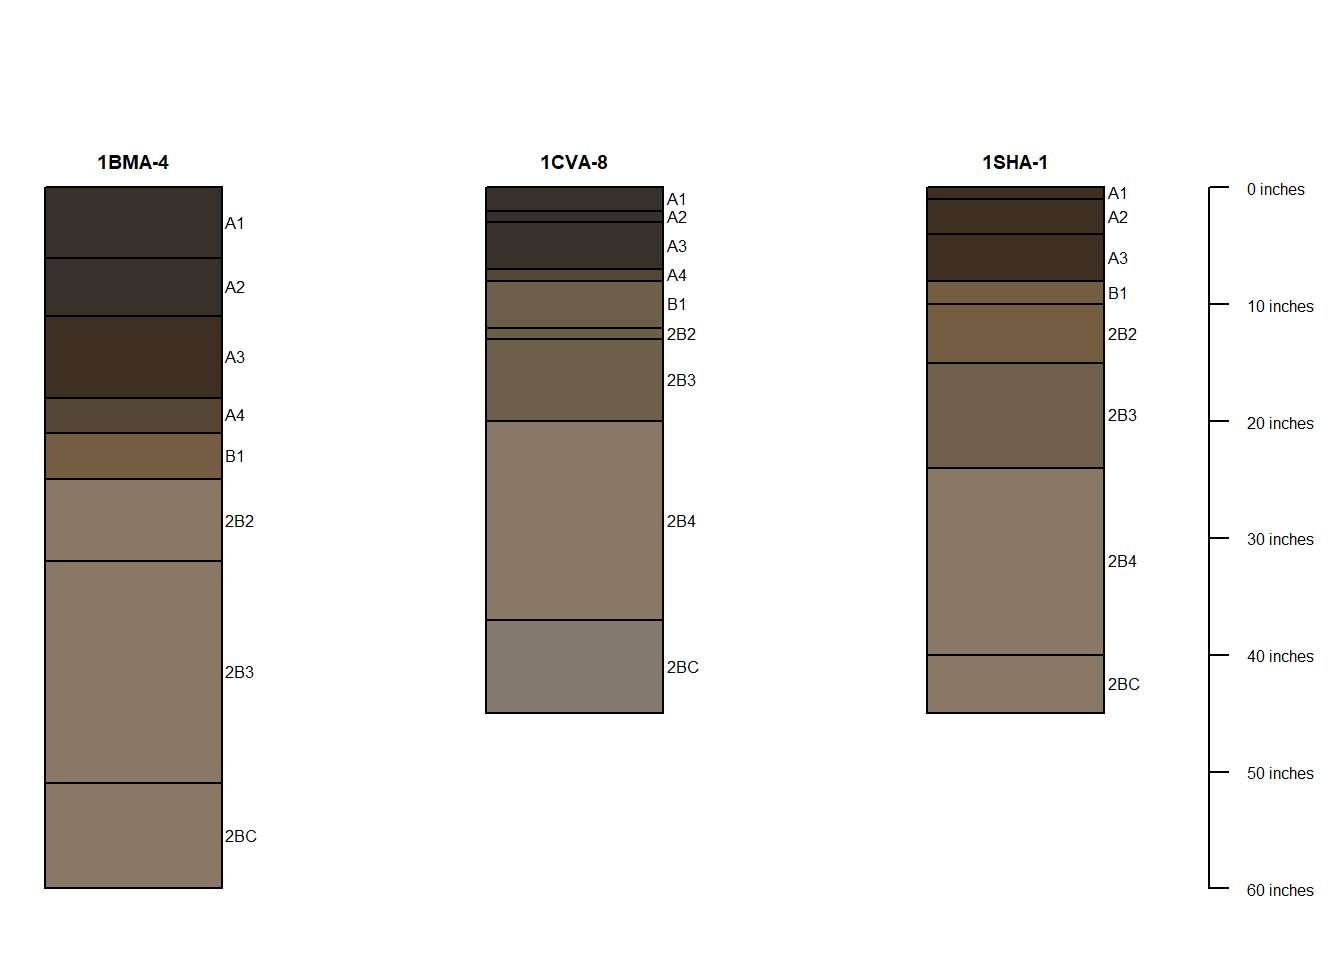
\includegraphics{bookdown-demo_files/figure-latex/unnamed-chunk-5-1.pdf}

\hypertarget{add-dashed-lines}{%
\section{Add dashed lines}\label{add-dashed-lines}}

Want to represent the lag line (transition to older till parent material) with a dotted line across each soil profile.

\begin{Shaded}
\begin{Highlighting}[]
\CommentTok{\# grab lag line depth from sites df}

\NormalTok{lag \textless{}{-}}\StringTok{ }\NormalTok{sites }\OperatorTok{\%\textgreater{}\%}\StringTok{ }
\StringTok{  }\KeywordTok{select}\NormalTok{(id, lag\_in)}

\CommentTok{\# need the ids in alpha order to align with pedons plotted alphabetically below (otherwise the lag lines get plotted on the wrong pedon).  Find a more robust solution for this in the future}

\NormalTok{lag\_sorted \textless{}{-}}\StringTok{ }\NormalTok{lag[}\KeywordTok{order}\NormalTok{(lag}\OperatorTok{$}\NormalTok{id),]}

\CommentTok{\# keep in mind that each pedon is centered over its integer index on the x{-}axis of the plot (first pedon centered over 1, second over 2, etc.)}
\NormalTok{x.pos \textless{}{-}}\StringTok{ }\DecValTok{1}\OperatorTok{:}\KeywordTok{length}\NormalTok{(with\_colors)}

\CommentTok{\# segments function needs vectors of coordinates:}
\CommentTok{\#specifies start/end the line segments}
\CommentTok{\# see https://bookdown.org/ndphillips/YaRrr/low{-}level{-}plotting{-}functions.html}
\NormalTok{from.x \textless{}{-}}\StringTok{ }\KeywordTok{c}\NormalTok{(x.pos }\OperatorTok{{-}}\StringTok{ }\FloatTok{0.2}\NormalTok{)}
\NormalTok{to.x \textless{}{-}}\StringTok{ }\KeywordTok{c}\NormalTok{(x.pos }\OperatorTok{+}\StringTok{ }\FloatTok{0.2}\NormalTok{)}
\NormalTok{from.y \textless{}{-}}\StringTok{ }\NormalTok{lag\_sorted}\OperatorTok{$}\NormalTok{lag\_in}
\NormalTok{to.y \textless{}{-}}\StringTok{ }\NormalTok{lag\_sorted}\OperatorTok{$}\NormalTok{lag\_in }

\KeywordTok{par}\NormalTok{(}\DataTypeTok{mar =} \KeywordTok{c}\NormalTok{(}\DecValTok{0}\NormalTok{,}\DecValTok{2}\NormalTok{,}\DecValTok{0}\NormalTok{,}\DecValTok{2}\NormalTok{))}

\KeywordTok{plot}\NormalTok{(with\_colors, }\DataTypeTok{name =} \StringTok{"name"}\NormalTok{,}
     \DataTypeTok{width =} \FloatTok{0.2}\NormalTok{)}

\KeywordTok{segments}\NormalTok{(}\DataTypeTok{x0 =}\NormalTok{ from.x,}
         \DataTypeTok{x1 =}\NormalTok{ to.x,}
         \DataTypeTok{y0 =}\NormalTok{ from.y,}
         \DataTypeTok{y1 =}\NormalTok{ to.y, }
         \DataTypeTok{col =} \StringTok{"red"}\NormalTok{, }
         \DataTypeTok{lwd =} \DecValTok{3}\NormalTok{, }\CommentTok{\# width of line}
         \DataTypeTok{lty =} \DecValTok{3}\NormalTok{)  }\CommentTok{\# line type}
\end{Highlighting}
\end{Shaded}

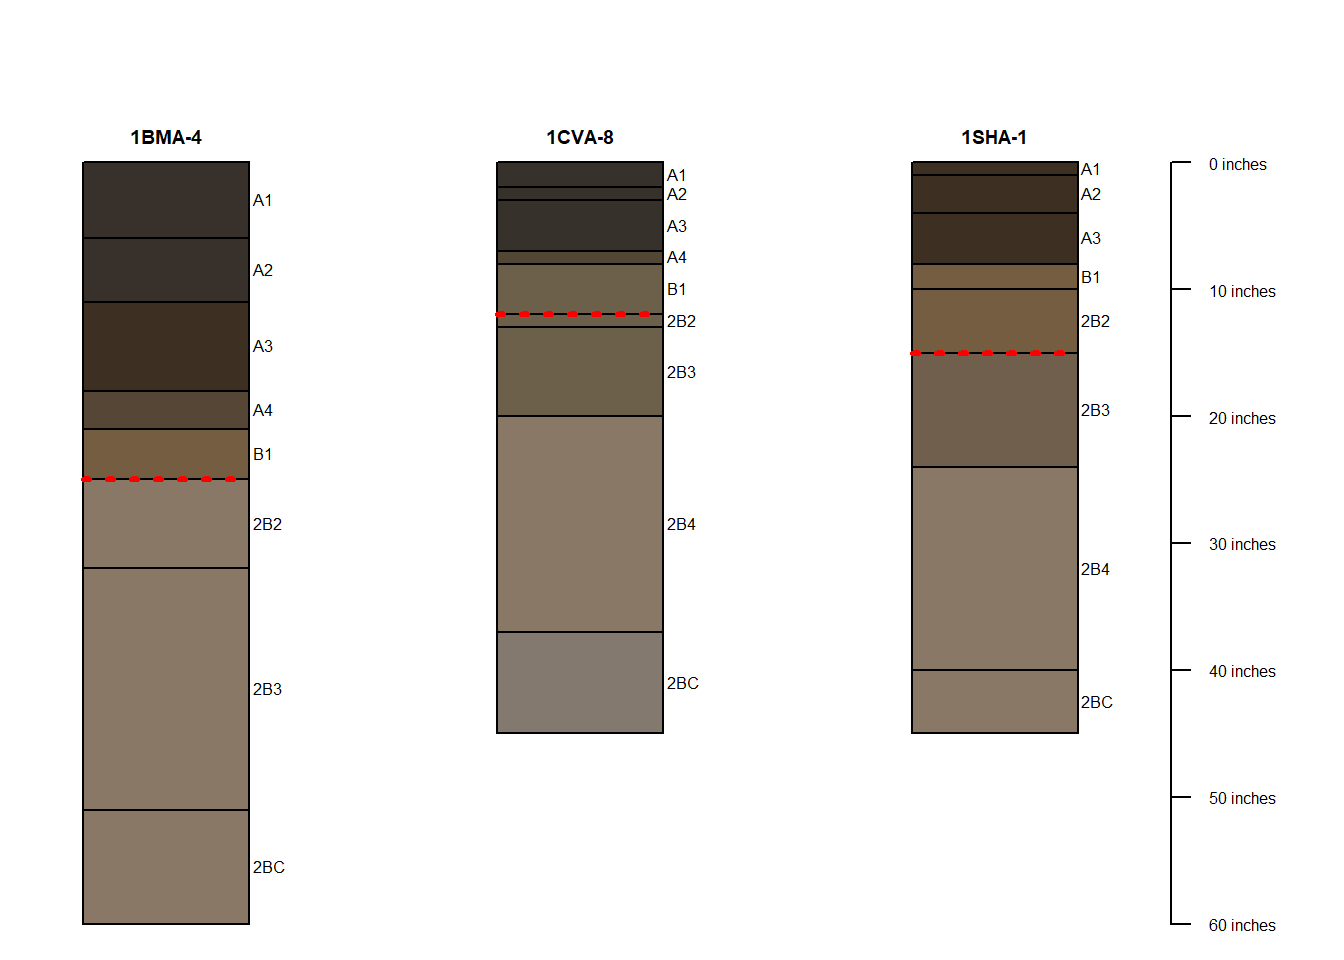
\includegraphics{bookdown-demo_files/figure-latex/unnamed-chunk-6-1.pdf}

\hypertarget{references}{%
\chapter{References}\label{references}}

Low level plotting functions, including segments() and text(), which might be useful for adding additional labels (such as ``lag line'') in the future: \url{https://bookdown.org/ndphillips/YaRrr/low-level-plotting-functions.html}

SPC plotting ideas:
\url{http://ncss-tech.github.io/AQP/aqp/SPC-plotting-ideas.html}

\begin{Shaded}
\begin{Highlighting}[]
\NormalTok{devtools}\OperatorTok{::}\KeywordTok{session\_info}\NormalTok{()}
\end{Highlighting}
\end{Shaded}

\begin{verbatim}
## - Session info -------------------------------------------------------------------------------
##  setting  value                       
##  version  R version 3.6.3 (2020-02-29)
##  os       Windows >= 8 x64            
##  system   x86_64, mingw32             
##  ui       RStudio                     
##  language (EN)                        
##  collate  English_United States.1252  
##  ctype    English_United States.1252  
##  tz       America/Chicago             
##  date     2020-09-06                  
## 
## - Packages -----------------------------------------------------------------------------------
##  package      * version  date       lib source        
##  aqp          * 1.19     2020-01-24 [1] CRAN (R 3.6.3)
##  assertthat     0.2.1    2019-03-21 [1] CRAN (R 3.6.3)
##  backports      1.1.8    2020-06-17 [1] CRAN (R 3.6.3)
##  blob           1.2.1    2020-01-20 [1] CRAN (R 3.6.3)
##  bookdown       0.20     2020-06-23 [1] CRAN (R 3.6.3)
##  broom          0.7.0    2020-07-09 [1] CRAN (R 3.6.3)
##  callr          3.4.3    2020-03-28 [1] CRAN (R 3.6.3)
##  cellranger     1.1.0    2016-07-27 [1] CRAN (R 3.6.3)
##  cli            2.0.2    2020-02-28 [1] CRAN (R 3.6.3)
##  cluster        2.1.0    2019-06-19 [2] CRAN (R 3.6.3)
##  codetools      0.2-16   2018-12-24 [2] CRAN (R 3.6.3)
##  colorspace     1.4-1    2019-03-18 [1] CRAN (R 3.6.1)
##  crayon         1.3.4    2017-09-16 [1] CRAN (R 3.6.3)
##  curl           4.3      2019-12-02 [1] CRAN (R 3.6.3)
##  DBI            1.1.0    2019-12-15 [1] CRAN (R 3.6.3)
##  dbplyr         1.4.4    2020-05-27 [1] CRAN (R 3.6.3)
##  desc           1.2.0    2018-05-01 [1] CRAN (R 3.6.3)
##  devtools       2.3.0    2020-04-10 [1] CRAN (R 3.6.3)
##  digest         0.6.25   2020-02-23 [1] CRAN (R 3.6.3)
##  dplyr        * 1.0.0    2020-05-29 [1] CRAN (R 3.6.3)
##  ellipsis       0.3.1    2020-05-15 [1] CRAN (R 3.6.3)
##  evaluate       0.14     2019-05-28 [1] CRAN (R 3.6.3)
##  fansi          0.4.1    2020-01-08 [1] CRAN (R 3.6.3)
##  forcats      * 0.5.0    2020-03-01 [1] CRAN (R 3.6.3)
##  formatR        1.7      2019-06-11 [1] CRAN (R 3.6.3)
##  fs             1.4.2    2020-06-30 [1] CRAN (R 3.6.3)
##  generics       0.0.2    2018-11-29 [1] CRAN (R 3.6.3)
##  ggplot2      * 3.3.2    2020-06-19 [1] CRAN (R 3.6.3)
##  glue           1.4.1    2020-05-13 [1] CRAN (R 3.6.3)
##  gtable         0.3.0    2019-03-25 [1] CRAN (R 3.6.3)
##  haven          2.3.1    2020-06-01 [1] CRAN (R 3.6.3)
##  hms            0.5.3    2020-01-08 [1] CRAN (R 3.6.3)
##  htmltools      0.5.0    2020-06-16 [1] CRAN (R 3.6.3)
##  httr           1.4.1    2019-08-05 [1] CRAN (R 3.6.3)
##  jsonlite       1.7.0    2020-06-25 [1] CRAN (R 3.6.3)
##  knitr          1.29     2020-06-23 [1] CRAN (R 3.6.3)
##  lattice        0.20-41  2020-04-02 [1] CRAN (R 3.6.3)
##  lifecycle      0.2.0    2020-03-06 [1] CRAN (R 3.6.3)
##  lubridate      1.7.9    2020-06-08 [1] CRAN (R 3.6.3)
##  magrittr       1.5      2014-11-22 [1] CRAN (R 3.6.3)
##  MASS           7.3-51.6 2020-04-26 [1] CRAN (R 3.6.3)
##  memoise        1.1.0    2017-04-21 [1] CRAN (R 3.6.3)
##  modelr         0.1.8    2020-05-19 [1] CRAN (R 3.6.3)
##  munsell      * 0.5.0    2018-06-12 [1] CRAN (R 3.6.3)
##  pillar         1.4.6    2020-07-10 [1] CRAN (R 3.6.3)
##  pkgbuild       1.1.0    2020-07-13 [1] CRAN (R 3.6.3)
##  pkgconfig      2.0.3    2019-09-22 [1] CRAN (R 3.6.3)
##  pkgload        1.1.0    2020-05-29 [1] CRAN (R 3.6.3)
##  plotrix        3.7-8    2020-04-16 [1] CRAN (R 3.6.3)
##  plyr           1.8.6    2020-03-03 [1] CRAN (R 3.6.3)
##  prettyunits    1.1.1    2020-01-24 [1] CRAN (R 3.6.3)
##  processx       3.4.3    2020-07-05 [1] CRAN (R 3.6.3)
##  ps             1.3.3    2020-05-08 [1] CRAN (R 3.6.3)
##  purrr        * 0.3.4    2020-04-17 [1] CRAN (R 3.6.3)
##  R6             2.4.1    2019-11-12 [1] CRAN (R 3.6.3)
##  raster         3.3-7    2020-06-27 [1] CRAN (R 3.6.3)
##  RColorBrewer   1.1-2    2014-12-07 [1] CRAN (R 3.6.0)
##  Rcpp           1.0.5    2020-07-06 [1] CRAN (R 3.6.3)
##  readr        * 1.3.1    2018-12-21 [1] CRAN (R 3.6.3)
##  readxl       * 1.3.1    2019-03-13 [1] CRAN (R 3.6.3)
##  remotes        2.1.1    2020-02-15 [1] CRAN (R 3.6.3)
##  reprex         0.3.0    2019-05-16 [1] CRAN (R 3.6.3)
##  reshape        0.8.8    2018-10-23 [1] CRAN (R 3.6.3)
##  reshape2       1.4.4    2020-04-09 [1] CRAN (R 3.6.3)
##  rlang          0.4.7    2020-07-09 [1] CRAN (R 3.6.3)
##  rmarkdown      2.3      2020-06-18 [1] CRAN (R 3.6.3)
##  rprojroot      1.3-2    2018-01-03 [1] CRAN (R 3.6.3)
##  rstudioapi     0.11     2020-02-07 [1] CRAN (R 3.6.3)
##  rvest          0.3.5    2019-11-08 [1] CRAN (R 3.6.3)
##  scales         1.1.1    2020-05-11 [1] CRAN (R 3.6.3)
##  sessioninfo    1.1.1    2018-11-05 [1] CRAN (R 3.6.3)
##  soilDB       * 2.5      2020-01-28 [1] CRAN (R 3.6.3)
##  sp             1.4-2    2020-05-20 [1] CRAN (R 3.6.3)
##  stringi        1.4.6    2020-02-17 [1] CRAN (R 3.6.2)
##  stringr      * 1.4.0    2019-02-10 [1] CRAN (R 3.6.3)
##  testthat       2.3.2    2020-03-02 [1] CRAN (R 3.6.3)
##  tibble       * 3.0.3    2020-07-10 [1] CRAN (R 3.6.3)
##  tidyr        * 1.1.0    2020-05-20 [1] CRAN (R 3.6.3)
##  tidyselect     1.1.0    2020-05-11 [1] CRAN (R 3.6.3)
##  tidyverse    * 1.3.0    2019-11-21 [1] CRAN (R 3.6.3)
##  usethis        1.6.1    2020-04-29 [1] CRAN (R 3.6.3)
##  vctrs          0.3.2    2020-07-15 [1] CRAN (R 3.6.3)
##  withr          2.2.0    2020-04-20 [1] CRAN (R 3.6.3)
##  xfun           0.15     2020-06-21 [1] CRAN (R 3.6.3)
##  xml2           1.3.2    2020-04-23 [1] CRAN (R 3.6.3)
##  yaml           2.2.1    2020-02-01 [1] CRAN (R 3.6.2)
## 
## [1] C:/Users/Hava/Documents/R/win-library/3.6
## [2] C:/Program Files/R/R-3.6.3/library
\end{verbatim}

  \bibliography{book.bib,packages.bib}

\end{document}
